
\subsubsection{Abbreviated Table Walk}

It is expected that the table walk will incur additional latency in the memory transaction
by the device. Certain device may be less tolerant of the latency, therefore, the IOMMU
provides an abbreviated address table walk to reduce the number of loads.

The Translation Descriptor is expanded with an entry, called \textit{Shortcut Table
Pointer}, that has the identical format as the
active paging mode. The PPN bits contains the physical address of the address table where
the look up should begin. The lower bits indicates which level of address table it points
to, so that the IOMMU is able to use the correct bits in the input address to index the
table. Figure \ref{fig:atw} illustrate this process.

\begin{figure}[ht!]
    \centering
    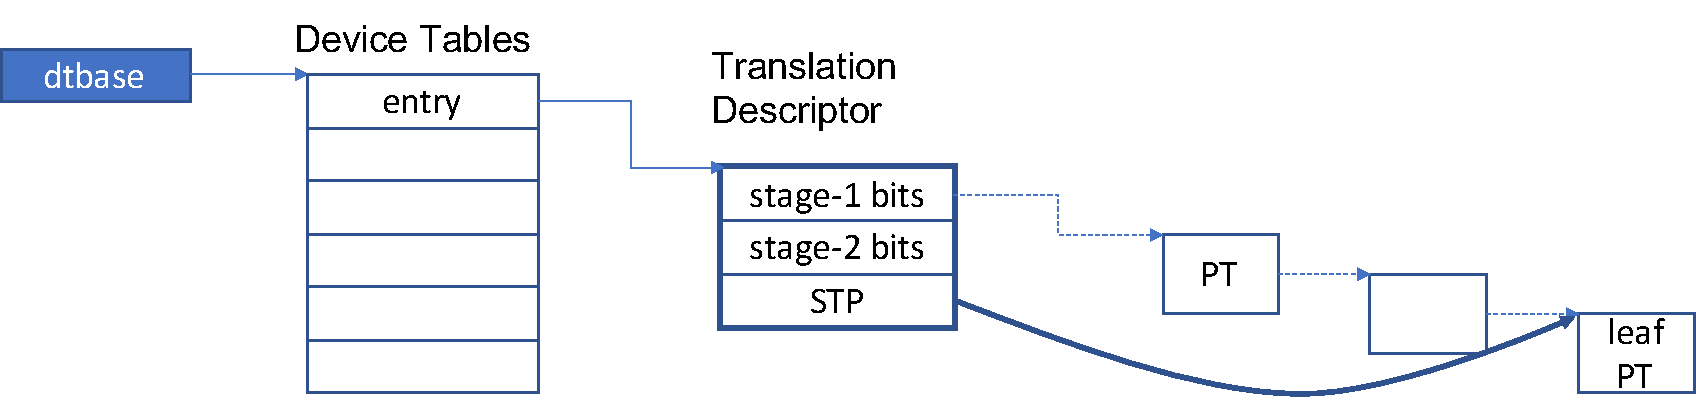
\includegraphics[width=0.95\textwidth]{img/atw.pdf}
    \caption{Abbreviated Table Walk for One Stage Translation}
    \label{fig:atw}
\end{figure}

The trade-off here is that the virtual address range that the device is able to access is
limited to the range that is mapped by the address table pointed to by the shortcut table
pointer.  This limitation is acceptable since the software will limit the address range
accessible by the device to it's own buffer anyway.

\note The observation is that once allocated, the addresses of the page table usually do
not change since they are kernel space data structures. Therefore, the software is able to
reliably use the address of the leaf table or the non-root, non-leaf tables. \noteend

